\chapter{ผลการทดลอง}

\section{ข้อมูลการทดลอง}
ในส่วนของการทดลองเชิงประจักษ์จะใช้ข้อมูลสองชนิดคือ ยูสเซอร์เบสเป็นข้อมูลโปรไฟล์ผู้ใช้จากเว็บไซต์ลิงค์อิน(linkedin) จำนวน 2,720 คน และตำแหน่งงานจากเว็บไซต์อินดีด(indeed) จำนวน 4,748 ตำแหน่ง โดยใช้คำสำคัญในการค้นหาข้อมูลจำนวนทั้งสิ้น 62 คำซึ่งเป็นตำแหน่งงานทางไอทีที่อิงจากสายงานทั้งหมด 8 สายงาน
\subsection{ข้อมูลโปรไฟล์ผู้ใช้}
ข้อมูลโปรไฟล์ผู้ใช้จะถูกสกัดโดยตรงจากเว็บไซต์ลิงค์อินโดยสกัดออกมาในรูปแบบเจสัน(json) และถูกนำมาแปลงเป็นรูปแบบตารางในขั้นตอนของการเตรียมการข้อมูลเพื่อบันทึกลงฐานข้อมูล จำนวนข้อมูลทั้งหมดที่สกัดมาจากเว็บไซต์ลิงค์อินคือ 2,720 คน
\newline
\begin{figure}[!h]
  \centering
  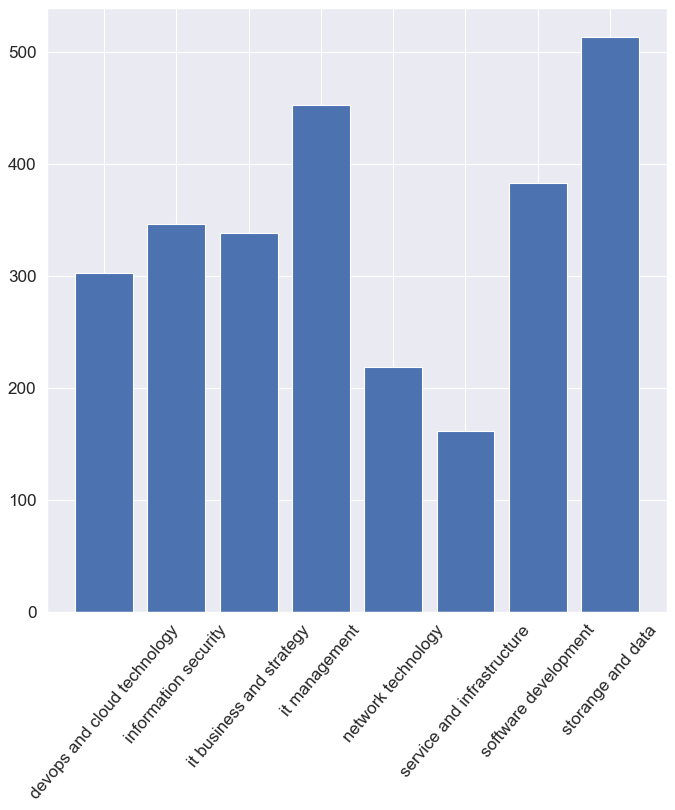
\includegraphics[width=0.7\textwidth]{chapter4/profile_graph.png}  
  \caption{ตารางเปรียบเทียบจำนวนโปรไฟล์ในแต่ละสายงาน}
  \label{Fig:result-profile-group}
\end{figure}

\begin{figure}[!h]
  \centering
  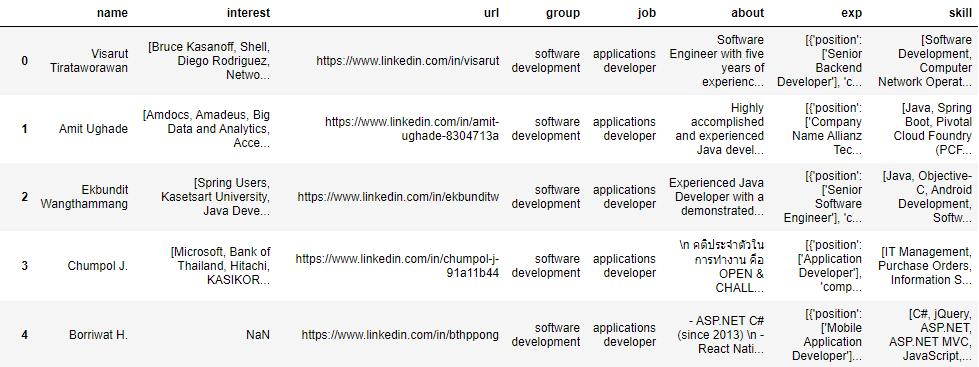
\includegraphics[width=1\textwidth]{chapter4/profile_data_table.jpg}  
  \caption{ตัวอย่างข้อมูลโปรไฟล์เปลี่ยนจากรูปแบบเจสันมาเป็นรูปแบบตาราง}
  \label{Fig:result-profile-group}
\end{figure}
\begin{figure}[!h]
  \centering
  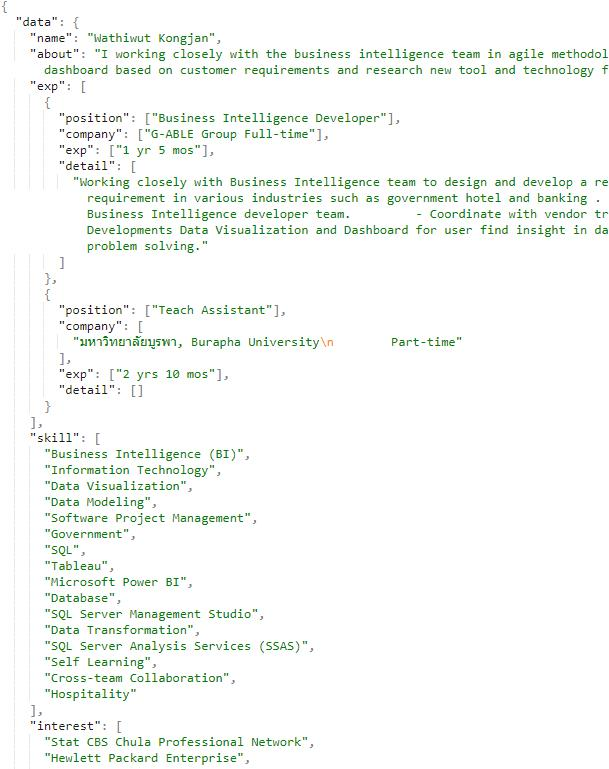
\includegraphics[width=0.8\textwidth]{chapter4/profile_data_json.jpg}  
  \caption{ตัวอย่างข้อมูลโปรไฟล์ที่ถูกสกัดมาในรูปแบบเจสัน}
  \label{Fig:result-profile-group}
\end{figure}
\clearpage

\subsection{ข้อมูลตำแหน่งงาน}
ข้อมูลตำแหน่งงานจะถูกสกัดมาจากเว็บไซต์อินดีด(indeed) ผ่านการส่งคำร้องไปที่เซิร์ฟเวอร์โดยตรงทำให้ง่ายต่อการได้มาของข้อมูล โดยข้อมูลที่สกัดมานั้นจะอยู่ในรูปแบบตารางจำนวนทั้งสิ้น 4,748 ตำแหน่ง
\begin{figure}[!h]
  \centering
  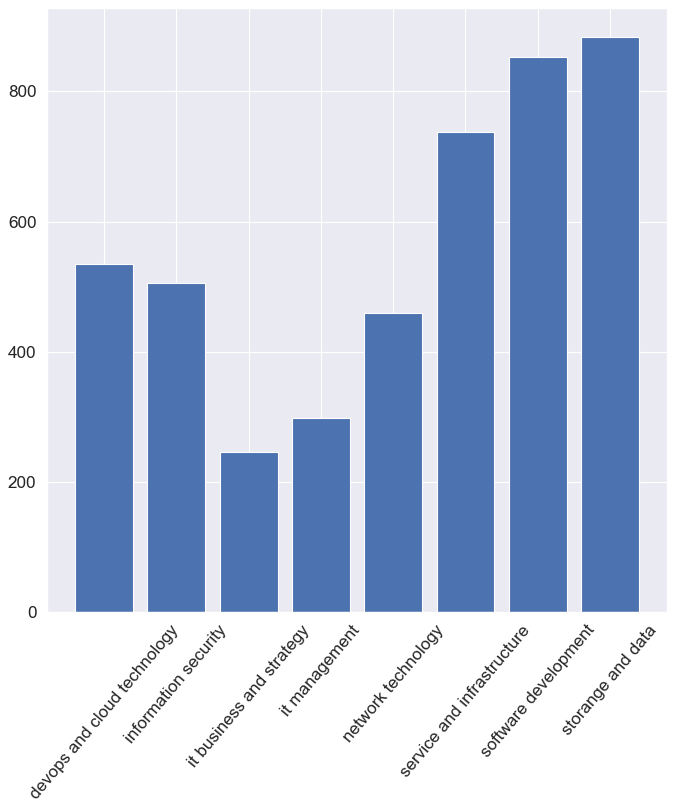
\includegraphics[width=0.7\textwidth]{chapter4/job_graph.png}  
  \caption{ตารางเปรียบเทียบจำนวนตำแหน่งงานในแต่ละสายงาน}
  \label{Fig:result-profile-group}
\end{figure}
\begin{figure}[!h]
  \centering
  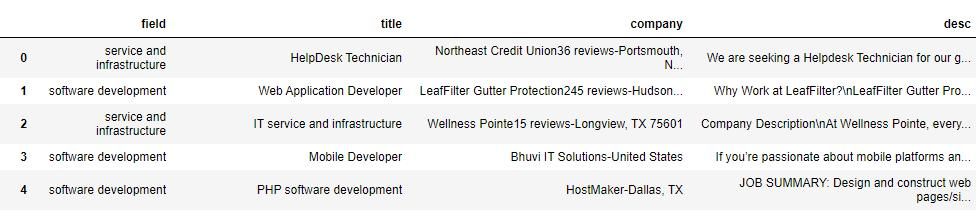
\includegraphics[width=1\textwidth]{chapter4/job_data_table.jpg}  
  \caption{ตัวอย่างข้อมูลตำแหน่งงานที่ถูกสกัดมาในรูปแบบตาราง}
  \label{Fig:result-profile-group}
\end{figure}


\section{การทำนายกลุ่มสายงาน}
\label{chapter:result}

ในการทำนายสายงานจะใช้โมเดลการเรียนรู้ของเครื่องจักรมาใช้ในการแบ่งแยกประเภทของสายงานทางไอทีซึ่งมาทั้งหมด 8 สายงานและใช้ข้อมูลโปรไฟล์ผู้ใช้เป็นยูสเซอร์เบส และข้อมูลตำแหน่งงานเป็นคอนเท้นเบส โดยใช้ทั้งสองข้อมูลนี้มาเทรนมาเทรนโมเดลแยกกัน เพื่อความหลายหลายในการแนะนำและแก้ปัญหาความคลุมเครือระหว่างสายงาน เช่น สายงาน devops and cloud technology ซึ่งทำงานใกล้ชิดกับฮาร์ดแวร์และการวางระบบต่าง ๆ ซึ่งใกล้เคียงอย่างมากกับสายงาน service and infrastructure ที่มีหน้าที่วางระบบและซัพพอร์ทเซอร์วิสต่าง ๆ \par
เทคนิคการการสร้างโครงสร้างของคำผู้จัดทำได้เลือกเทคนิค TFIDF ซึ่งจากการเปรียบเทียบกับเทคนิคอื่นๆ เช่น word2vec หรือ word vectorizer แล้วเทคนิค TFIDF ให้ค่าความแม่นยำที่สูงที่สุดและเมื่อดูจากการกระจายตัวของคำในกราฟแล้วจะเห็นว่า TFIDF มีการกระจายตัวของกลุ่มที่เหตุชัดมากที่สุด 
ต่อมาคือเทคนิคที่ใช้ในการเทรนโมเดล NLP จะใช้เทคนิค "support vector machine" มาใช้ในการเทรนโมเดล เนื่องจากมีความแม่นยำสูงสุดเมื่อเทียบกับเทอื่นๆ เช่น "logistic regress" และมีผลลัพธ์ดังนี้

\subsection{ยูสเซอร์เบส}
ยูสเซอร์เบสเป็นการใช้ข้อมูลโปรไฟล์ผู้ใช้มาใช้เป็นฐานในการเทรนโมเดลและทำนายตำแหน่งงานจะสรุปได้ดังนี้

\begin{figure}[!h]
  \centering
  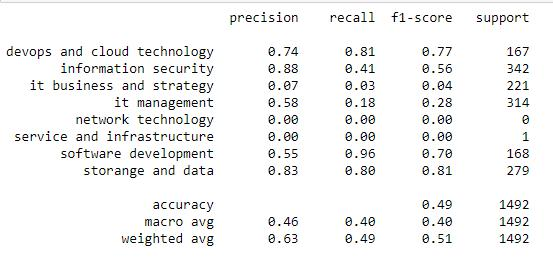
\includegraphics[width=0.8\textwidth]{chapter4/profile_report.jpg}  
  \caption{รายงานการแบ่งกลุ่มโดยใช้ข้อมูลโปรไฟล์}
  \label{Fig:result-profile-group}
\end{figure}
จากการวิเคราะห์จะคาดการได้ว่าโปรไฟล์ผู้ใช้ลิงค์อินนั้นมีความแม่นยำที่ค่อนข้างต่ำ โดยมีความแม่นยำอยู่ที่ 49\% ซึ่งเหตุผลอาจเป็นเพราะผู้ใช้มักใส่ทักษะวิชาชีพครอบคลุมทุกสิ่งที่อย่างที่รู้จักโดยไม่คำนึงว่าผู้ใช้นั้นมีความเชียวชาญหรือไม่ และในส่วนของคำอธิบายส่วนตัว ผู้ใช้บางส่วนไม่ได้เขียนถึงความเชี่ยวชาญหรือการทำงานของตนเองแต่อาจเขียนถึงสิ่งที่ไม่เกี่ยวกับสิ่งที่ทำเลย เช่น การแนะนำตัวบอกถึงสิ่งที่ชอบสิ่งที่รักหรือกลอน เป็นต้น

\begin{figure}[!h]
  \centering
  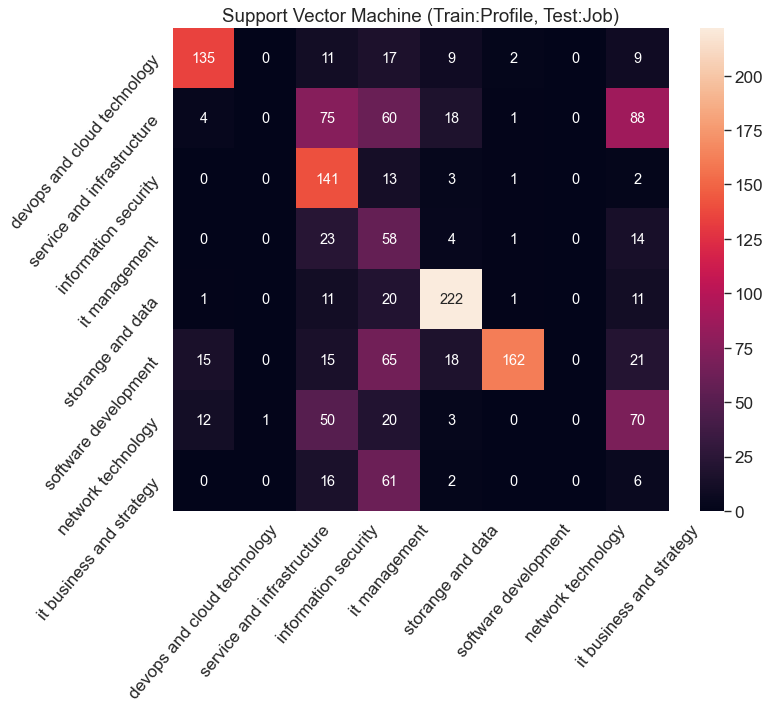
\includegraphics[width=0.8\textwidth]{chapter4/profile_confusion.png}  
  \caption{confusion matrix จากการทำนายโดยใช้ข้อมูลโปรไฟล์ผู้ใช้}
  \label{Fig:result-profile-group}
\end{figure}
\begin{figure}[!h]
  \centering
  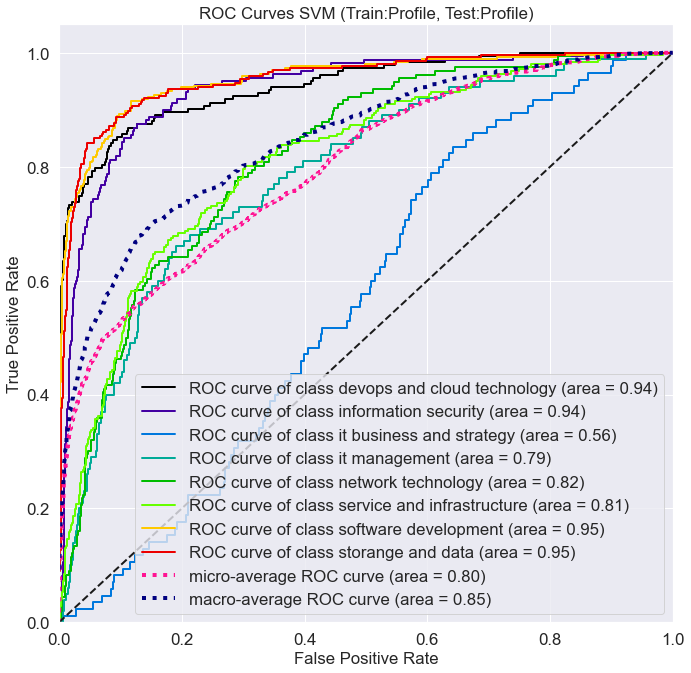
\includegraphics[width=0.7\textwidth]{chapter4/profile_roc.png}  
  \caption{ตาราง roc จากการทำนายโดยใช้ข้อมูลตำแหน่งงาน}
  \label{Fig:result-profile-group}
\end{figure}
\clearpage

\subsection{จ็อบเบส}
จ็อบเบสการใช้ข้อมูลตำแหน่งงานมาใช้เป็นฐานในการเทรนโมเดลและทำนายตำแหน่งงานจะสรุปได้ดังนี้

\begin{figure}[!h]
  \centering
  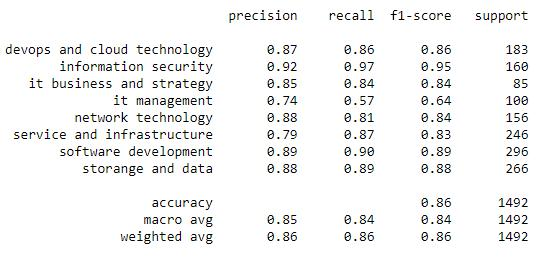
\includegraphics[width=0.8\textwidth]{chapter4/job_report.jpg}
  \caption{รายงานการแบ่งกลุ่มโดยใช้ข้อมูลโปรไฟล์}
  \label{Fig:result-profile-group}
\end{figure}
การใช้ข้อมูลตำแหน่งงานหรือจ็อบเบสมาใช้ในการเทรนโมเดลจะเห็นว่าตัวโมเดลมีความแม่นยำเป็นอย่างมากโดย ความแม่นยำอยู่ที่ 89\% จารการวิเคราะห์จะพบว่าเนื่องจากเนื้อหาของตำแหน่งงานเป็นสิ่งที่ค่อนข้างตายตัวในตัวของเนื้อหาอยู่แล้ว เช่นในสายงานของ software development ตำแหน่งงานส่วนใหญ่จะเขียนความต้องการเป็นภาษาที่สามารถเขียนได้เป็นต้น

\begin{figure}[!h]
  \centering
  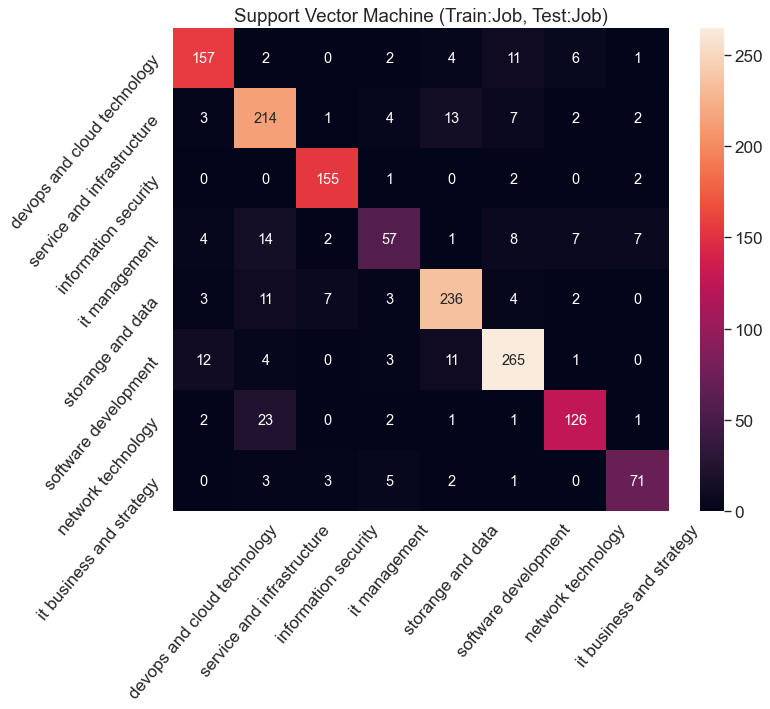
\includegraphics[width=0.8\textwidth]{chapter4/job_confusion.png}  
  \caption{confusion matrix จากการทำนายโดยใช้ข้อมูลตำแหน่งงาน}
  \label{Fig:result-profile-group}
\end{figure}
\begin{figure}[!h]
  \centering
  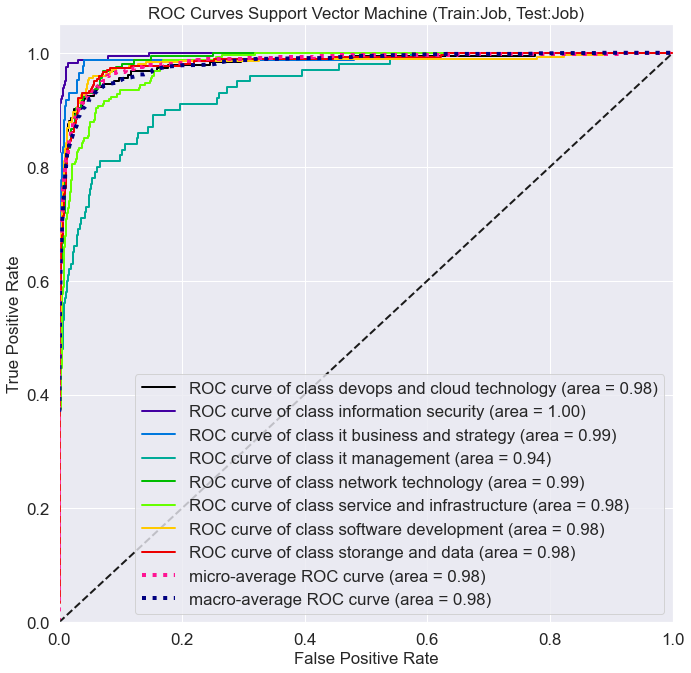
\includegraphics[width=1\textwidth]{chapter4/job_roc.png}  
  \caption{ตาราง roc จากการทำนายโดยใช้ข้อมูลตำแหน่งงาน}
  \label{Fig:result-profile-group}
\end{figure}
\clearpage

\newpage
\section{ระบบแนะนำ}
ในขั้นตอนแนะนำตำแหน่งานข้อมูลนำเข้าจากผู้ใช้ที่ต้องการตำแหน่งงานที่เหมาะสมกับโปรไฟล์จะถูกนำมาใช้ในการหาระยะทางโคไซน์ โดยขั้นตอนนี้จำเป็นต้องใช้ทรัพย์ยากรเครื่องจำนวนมาก ด้วยเหตุนี้ระบบแนะนำผลของการแบ่งกลุ่มสายงาน มาใช้ในการแบ่งข้อมูลตำแหน่งงานที่มีอยู่เพื่อลดปริมาณข้อมูลที่ต้องคำนวน และเวลาที่ใช้ในการรอผลลัพธ์ \newline
โดยผลลัพธ์ของการแนะนำตำแหน่งงานจะแสดงเรียงตามคว้ามคล้ายคลึงกันระหว่างโปรไฟล์ผู้ใช้ของเรา กับตำแหน่งงานทั้งหมดที่ถูกแบ่งโดยขั้นตอนแบ่งกลุ่มสายงาน ผลลัพธ์ที่แสดงออกมาจากการตอบกลับของเอพีไอจะเป็นดังนี้

\paragraph*{คำร้อง}
  payload ของข้อมูลที่ส่งไปกับคำร้องคือไฟล์ผู้ใช้ที่ต้องการหางานที่เหมาะสมโดยอยู่ในรูปแบบ json ดังนี้
  \begin{figure}[!h]
    \centering
    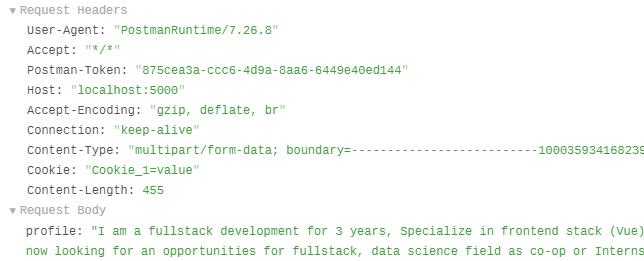
\includegraphics[width=1\textwidth]{chapter4/recomm_request.jpg}  
    \caption{ตัวอย่างคำร้องแนะนำตำแหน่งงาน}
    \label{Fig:recomm_request}
  \end{figure}
  \clearpage

\paragraph*{คำตอบรับ}
  ข้อมูลที่ตอบกลับมาจากเซิร์ฟเวอร์จะเป็นข้อมูลรายการตำแหน่งงานที่อยู่ในรูปแบบ json ดังนี้
  \begin{figure}[!h]
    \centering
    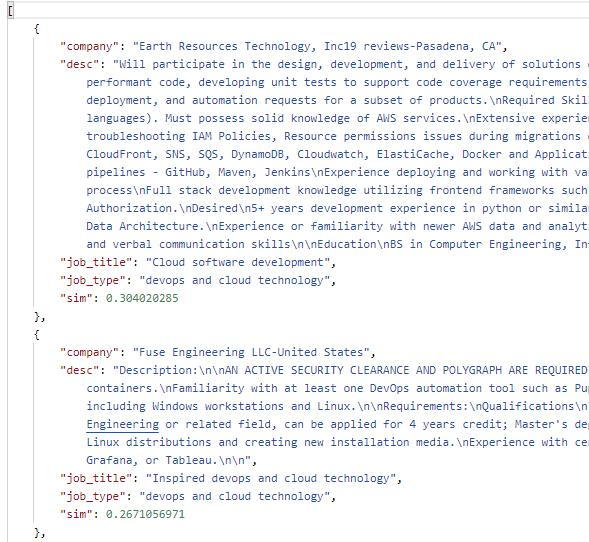
\includegraphics[width=1\textwidth]{chapter4/recomm_response.jpg}  
    \caption{ตัวอย่างคำตอบรับแนะนำตำแหน่งงาน}
    \label{Fig:recomm_response}
  \end{figure}
  \clearpage

\section{เว็บให้บริการระบบแนะนำ}
  \paragraph*{แบบฟอร์ม} แบบฟอร์มสำหรับกรอกข้อมูลโปรไฟล์ผู้ใช้เพื่อนำข้อมูลนี้มาใช้ในการจับคู่ตำแหน่งงานที่เหมาะสม
  \begin{figure}[!h]
    \centering
    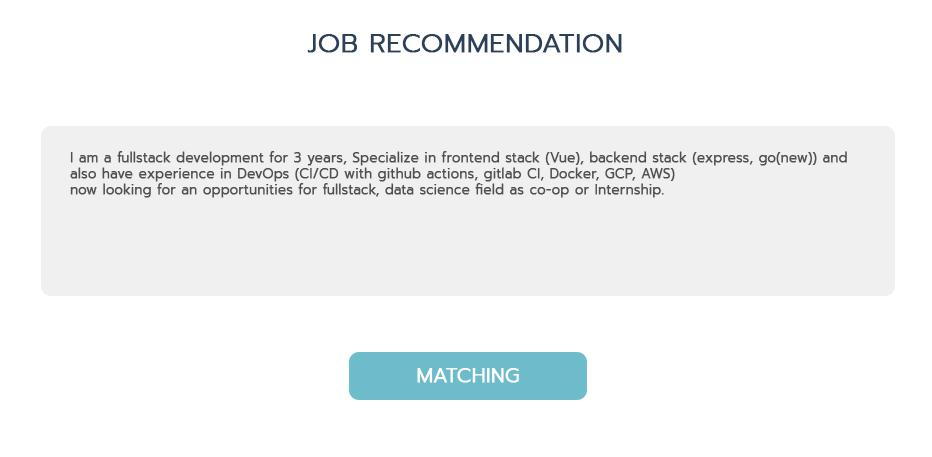
\includegraphics[width=1\textwidth]{chapter4/frontend_form.jpg}  
    \caption{แบบฟอร์มสำหรับกรอกข้อมูลโปรไฟล์ผู้ใช้}
    \label{Fig:frontend_form}
  \end{figure}

  \paragraph*{ตำแหน่งงาน} รายการตำแหน่งงานที่เหมาะสมกับโปรไฟล์ผู้ใช้
  \begin{figure}[!h]
    \centering
    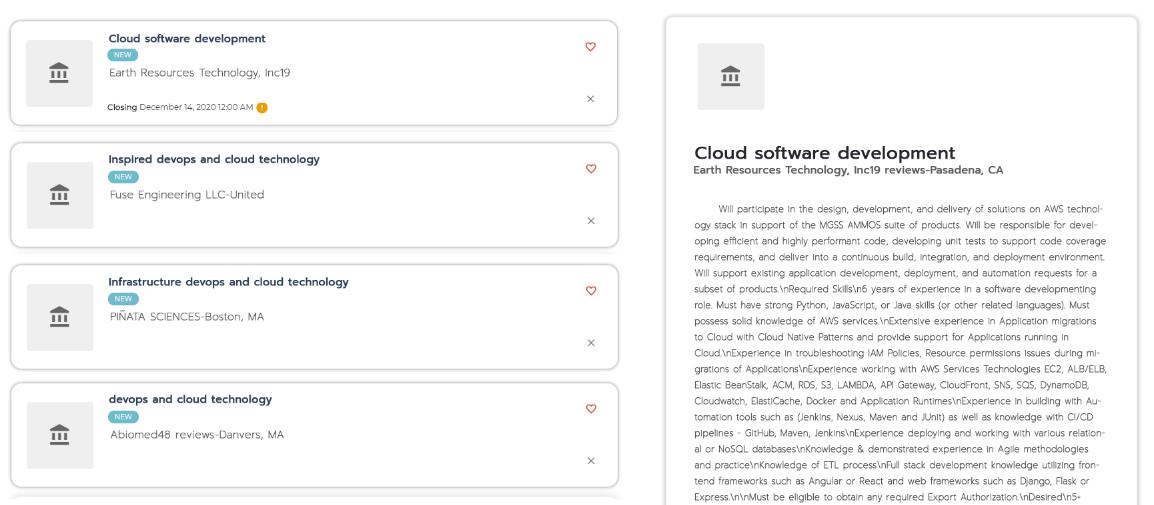
\includegraphics[width=1\textwidth]{chapter4/frontend_response.jpg}  
    \caption{รายการตำแหน่งงานที่ถูกแนะนำ}
    \label{Fig:frontend_form}
  \end{figure}

